% -*- root: ../main.tex -*-
%!TEX root = ../main.tex
% this file is called up by main.tex
% content in this file will be fed into the main document
% vim:textwidth=80 fo=cqt

\clearpage
\chapter{Introduction}\label{ch:intro}

More introductory material goes here blah blah \dots \dots

In recent years, tightening emissions regulations for various industrial sectors
have  forced a  renewed interest  in sustainable  energy sources{[}cite{]}.  The
demand  for  clean  energy  has  led  the  automotive,  utilities  and  consumer
electronics industries to develop  advanced methods of storing energy{[}cite{]}.
Li-ion batteries  are seen as key  enablers in this quest  {[}cite{]} ; however,
with this explosion  in energy storage requirements comes a  stricter demand for
cell  longevity, performance,  and adhesion  to safety  requirements {[}cite{]}.
Lithium-ion cells have several advantages over other cell compositions including
high  energy density,  extended lifecycle,  low internal  resistance, low  self-
discharge, long cycle  life, fast charge and discharge  cycles {[}cite{]} making
it no surprise that nearly all  modern consumer electronics and electric vehicle
(EV) manufacturers  employ this technology  to varying degrees in  their product
portfolio.

Through  accurate  model representations  of  the  electrochemical behaviour  of
the  cell,  advanced  control  strategies   can  be  deployed  to  tackle  these
challenges{[}cite{]}. With safety and performance being of utmost concern, extra
efforts have  been made to  construct accurate  models to describe  the physical
behavior  of  the  cell  {[}cite{]}.Modern  demand  for  increased  performance,
operating  lifecycle   and  safety  of   batteries  has  led   to  sophisticated
modeling strategies.  These models  govern the  operation of  Battery Management
Systems  (BMS) in  various  applications ranging  from  portable electronics  to
automotive. Most  models have  the primary intent  of accurately  estimating the
cell\textquoteright s voltage and  state-of-charge;more advanced models give key
insight into  physical parameters that could  affect the health of  the battery.
The literature on Li-ion battery modelling  can be generally classified into two
broad  approaches  : (1)  Empirical/Ad-hoc  equivalent  circuit models  and  (b)
Detailed  Physics-Based  models  based  upon first  principles.  However,  these
two  approaches  are generally  at  loggerheads  with  each  other in  terms  of
computational complexity as discussed below.

Equivalent  circuit  models  employ   circuit  elements  like  voltage  sources,
resistors  and capacitors  to  model  the general  behaviour  of batteries.  The
parameters of the circuit can be identified using numerical optimization methods
{[}cite{]}  or through  Electrochemical Impedance  Spectroscopy {[}cite{]}.  The
open-circuit  voltage and  capacity of  the  battery are  usually determined  by
measuring the terminal voltage and integrating the applied current during a very
slow discharge  test (eg. at a  C/30 rate). Using the  equivalent circuit model,
the cell\textquoteright  s state  of charge  (SOC) can  be calculated  using two
simple  methods  using discharge  test  data  -- a)  the  manufacturer-specified
OCV-SOC  lookup table  and  b)  coulomb counting  {[}cite{]}.  Both methods  are
computationally  amenable for  small-scale embedded  applications like  consumer
electronics;  however, neither  one  is robust  for  modern performance  demands
imposed  by vehicular  applications. More  advanced methods  which employ  these
equivalent circuit models, such as nonlinear Kalman filtering, produce very good
robust estimates  {[}9{]}. The usefulness  of the ECM  models is limited  by the
fact that  their parameters are  derived essentially by a  curve-fitting process
using training data.  Since they are not based on  any physical phenomena, their
ability to predict cell behavior is  extremely poor especially when applied with
current profiles outside the training realm.

Physics-based  models  employ governing  equations  that  construct an  accurate
realization  of  the   behaviour  of  the  system  based   on  first  principles
of   electrochemical   thermodynamics   and   kinetics.   Doyle,   Fuller,   and
Newman  {[}cite{]}   developed  a  porous   electrode  model  to   describe  the
cells\textquoteright{} internal variables like  solid and electrolyte potential,
solid  and   electrolyte  concentrations,   and  lithium  molar   flux  density,
respectively. The fundamental  advantage to this modelling approach  is that the
prediction  of the  internal variables  can  be obtained  for arbitrary  current
profiles, whereas the  error of the equivalent circuit models  is very high when
current profiles outside  the model\textquoteright s training  realm is applied.
Also, direct estimation  of state-of-charge and cell-capacity  is obtained using
the  Physics-based  model {[}cite{]}.  The  difficulty  with the  physics  based
modelling  approach is  to obtain  the values  of all  the physical,  geometric,
electrochemical, thermal  and kinetic  parameters of  the cells.  Usually, these
parameters are  trade secrets of various  cell manufacturers, and varies  due to
production spread.  Only a  limited number  of cell  parameters can  be obtained
directly from laboratory experiments. Hence,  some sort of system identification
method needs to be employed for extrapolating other cell parameters. Also, it is
a common practice to rely on published data for estimating certain parameters of
the cell that do not depend  on physical construction, especially for those that
remain universally  true for a particular  Li-ion family of cell  chemistry. The
disadvantage of physics-based models is that their simulation is time-consuming,
requiring  sophisticated  multi-physics  PDE  solvers and  hence  not  typically
suitable for  embedded applications. However, for  high performance applications
like automotive battery management  systems where the state-of-health monitoring
is crucial,  there is an overwhelming  demand for the insight  into the internal
cell variables. Thus, applying various model order reduction technqiues are seen
a key enabler in porting the predictive powers of the physics-based model into a
real-time microprocessor.




Ragone plot

Different type of cells - Prismatic,  pouch and cylindrical. How pouch cells are
used in automotive industry acknowledge Tesla, but cite counter citations. Layer
photos etc

This  thesis  strives to  represent  all  physical  quantities in  the  standard
International  System  of Units  (SI-Units).  However,  there are  some  notable
exceptions \eg{} for the capacity of a  Li-ion cell, which is represented in the
practical units  of Ampere  hours (\SI{}Ah),  rather than the  base SI  Units of
Coulombs (\SI{}{\coulomb}).  Such exceptions  are made  taking into  account the
prevalent conventions in standard literature.

\fxnote{make a note in the introduction  chapter that the terms cell and battery
are  used  interchangeably deviating  from  their  precise meaning,  \eg{}  cell
modelling and battery modelling}

% \cite{Grazioli2016a} goes crazy in reviewing the models out there.

% \cite{Seaman2014} provide a comprehensive survey  of the wide range of battery
% models out there.

Based on an isothermal description
Mention  that stuff  is  applicable for  both Lithium  ion  and Lithium  polymer
chemistries.


\section{Chemistry}\label{subsec:liionchemistry}

This section  provides a  brief overview of  the essential  chemistry principles
that helps to provide a background context for the governing equations presented
in~\cref{subsec:basicspmgoverningeqns}.


In  a Li-ion  cell,  the  positive electrode  consists  of  porous particles  of
Lithium-Transition Metal Oxide (MO)  compounds. The negative electrode typically
employs  some  variant  of  microporous  graphite.  The  porous  nature  of  the
electrodes provide pathways for lithium  ion conduction through the electrolyte.
Due  to  the  special  construction  of the  electrode  structure,  there  exist
interstitial  sites  which act  as  intercalation  spots for  Lithium  shuttling
between the two  electrodes. The electrolyte, whose dynamics are  ignored in the
\gls{spm}, helps  in the  conduction of \ch{Li^+}  ions. The  separator membrane
allows  the passage  of  these ions  between the  two  electrodes, but  prevents
internal  short-circuit  by inhibiting  electronic  conduction  through it.  The
current collectors facilitate  passage of electrons generated  during the charge
transfer reaction  at particle surface  to the  external circuit. With  the help
of~\cref{fig:chargetransferprocess}  the  steps  involved  in  this  process  is
detailed next.

\begin{figure}[!htbp]
    \centering
    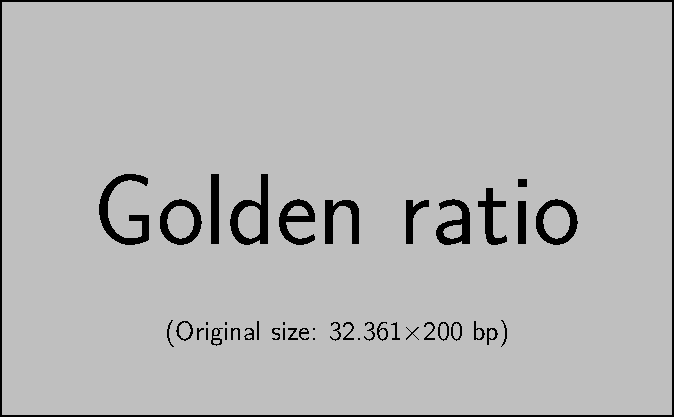
\includegraphics{placeholder_images/example-image-golden.pdf}
    \caption[Charge-transer and basic working mechanism of a Li-ion cell]{Simplified representation of charge-transfer
    process and illustration of basic working mechanism of a Li-ion cell.}
    \label{fig:chargetransferprocess}
\end{figure}

At fully  charged condition,  the majority  of Lithium in  the system  is stored
within  the  negative  electrode  microstructure.  During  discharge,  \ch{Li^0}
atoms  diffuse  out of  deep  interstitial  sites  towards  the surface  of  the
particles  in  the negative  electrode.  At  the surface  (electrode-electrolyte
interface),  a charge-transfer  process takes  place according  to Butler-Volmer
kinetics~\cref{eq:butlervolmer}, leading to the  formation of \ch{Li^+} ions and
electrons.  The electrons  are passed  to the  external circuit  through \ch{Cu}
current collectors  onto which  the conductive matrix  composed of  the negative
electrode material and binders is coated.  The \ch{Li^+} ions travel through the
electrolyte phase,  crossing the  separator membrane  to the  positive electrode
where they  encounter an  electron influx  from the  external circuit.  A charge
transfer  reaction  takes  place  at  the  surface  of  the  positive  electrode
particles, leading to the formation of neutral \ch{Li^0} atoms that diffuse into
the positive electrode microstructure.

During  the   charging  process,  the   reverse  phenomena  occur.   Lithium  is
de-intercalated  from  the  positive  electrode and  a  similar  charge-transfer
happens  at the  surface,  leading  to the  formation  of  \ch{Li^+} ions  which
reach  the  negative  electrode  by   passing  through  the  separator.  At  the
surface  of  the  negative  electrode particles,  these  ions  absorb  electrons
from  the  external circuit,  leading  to  the  formation of  neutral  \ch{Li^0}
that   diffuses  into   interior   vacant  spaces   in   the  layered   graphite
electrode. The  charge-transfer mechanism  and sequence  of events  are depicted
in~\cref{fig:chargetransferprocess}.
\Cref{eq:NegElectrodeRxn,eq:PosElectrodeRxn} summarise the reactions during the
charging and discharging process at the surfaces of both electrode materials.
\begin{align}
    \ch{Li_{$x$} C                            &<=>[\tiny{discharge}][\tiny{charge}] C + $x$ Li^+ + $x$ e^-}\label{eq:NegElectrodeRxn}\\
    \ch{Li_{1-$x$} M O2 + $x$ Li^+  + $x$ e^- &<=>[\tiny{discharge}][\tiny{charge}] LiMO2}\label{eq:PosElectrodeRxn}
\end{align}
where    \ch{M}   represents    a    transition   metal    compound   such    as
\ch{Ni_{1/3}Co_{1/3}Mn_{1/3}}   (NMC),   \ch{Ni_{0.8}Co_{0.15}Al_{0.05}}   (NCA)
amongst other  choices~\cite{Reddy2011}. Assuming  no loss of  cycleable Lithium
due to  parasitic side  reactions or  through other  mechanisms, the  process is
fully reversible.


The electrochemical potential at each electrode  is dependent upon the extent of
its  lithiation. An  empirical  relationship of  each  electrode's potential  as
a  function  of  its  stoichiometry  can be  obtained,  and  is  dependent  upon
the  specific design  and  material  properties of  each  active material  under
consideration. Finally, the \gls{ocv} of the cell is obtained by subtracting the
negative electrode potential from its positive electrode counterpart.

% -*- root: ../main.tex -*-
%!TEX root = ../main.tex
% this file is called up by main.tex
% content in this file will be fed into the main document
% vim:nospell textwidth=180 foldlevelstart=3 foldlevel=3

% \begin{table}[!htbp]
    \begin{table}[p]
        \centering
        \caption[]{}
        % \label{tbl:charSimspmp2d}
        \begin{threeparttable}
            \begingroup
            \makeatletter\def\f@size{10.0625}\check@mathfonts
            % \addtolength{\jot}{0.75em}
            \addtolength{\jot}{0.875em}
            \begin{tabular*}{\textwidth}{@{} l c r l r @{}}
                \toprule
                Region & Governing equations & \multicolumn{3}{c}{Boundary conditions} \\
                \midrule
                \multicolumn{1}{l |}{\rotatebox[origin=c]{+90}{\makecell{\small Electrodes \\ \small \linnegpos}}} &
                $\begin{aligned} % placement: default is "center", options are "top" and "bottom"
                    \vphantom{\diffp{c_\slsub}{r}{\mathrlap{r = R_\pl}}}
                    \diffp{c_\slsub}{t} &= \frac{D_\slsub}{r^2}\diffp{}{r}\left(r^2 \diffp{c_\slsub}{r} \right) \\
                    \vphantom{\diffp{c_\text{e}}{x}{\mathrlap{x = l_\text{tot}}}}
                    \varepsilon_l \diffp{c_\text{e}}{t} &= \diffp{}{x}\left(D_\effl
                    \diffp{c_\text{e}}{x} \right) + (1 - t^0_\text{+}) a_\slsub j_l \\
                    \vphantom{\diffp{\phi_\text{e}}{x}{\mathrlap{x = 0}}} 0 &= \diffp{}{x}\left(\kappa_\effl \diffp{\phi_\text{e}}{x}\right) + \diffp{}{x}\left(\kappa_\effl \frac{2 R T(t)}{F} (t^0_{+}-1)\diffp{ \ln c_\text{e}}{x}\right) \\
                    \vphantom{\sigma_\effl\!\diffp{\phi_\slsub}{x}{\mathrlap{\substack{\vphantom{\displaystyle M}x = x_\text{pos/sep}\\x = x_\text{neg/sep}}}}} a_\slsub F j_l &= \diffp{}{x}\left(\sigma_\effl \diffp{\phi_\slsub}{x}\right) \\
                    % j_l &= k_\lr c^\alpha_\text{e}\left(c_\slmax - c_\slsurf\right)^\alpha c^\alpha_\slsurf\left( \exp\left(\frac{\left(1-\alpha\right)F}{R T}\eta\right) - \exp\left(-\frac{\alpha F}{R T}\eta\right) \right)
                    j_l &= 2 k_\lr \sqrt{c_\text{e}\left(c_\slmax - c_\slsurf\right) c_\slsurf} \sinh \left(\frac{0.5 F}{R T(t)} \eta_l \right)
                \end{aligned}$ &
                $\begin{aligned}
                    \vphantom{\diffp{c_\slsub}{r}{\mathrlap{r = R_\pl}}} \diffp{c_\slsub}{r}{\mathrlap{r = 0}}\hspace{1mm} &= 0, \\
                    \vphantom{\diffp{c_\text{e}}{x}{\mathrlap{x = l_\text{tot}}}} \diffp{c_\text{e}}{x}{\mathrlap{x = 0}}\hspace{1mm} &= 0, \\
                    \diffp{\phi_\text{e}}{x}{\mathrlap{x = 0}}\hspace{1mm} &= 0, \\
                    \sigma_\effl\!\diffp{\phi_\slsub}{x}{\mathrlap{\substack{\vphantom{\displaystyle M}x = x_\text{pos/sep}\\x = x_\text{neg/sep}}}}\hspace{1mm} &= 0, \\
                    % {}&\textemdash{}{}
                    {}&\xdash[1.25em]{}
                \end{aligned}$ &
                $\begin{aligned}
                    \diffp{c_\slsub}{r}{\mathrlap{r = R_\pl}}\hspace{1mm} &= \frac{-j_l}{D_\slsub} \\
                    \diffp{c_\text{e}}{x}{\mathrlap{x = l_\text{tot}}}\hspace{1mm} &= 0 \\
                \vphantom{\diffp{\phi_\text{e}}{x}{\mathrlap{x = 0}}} \phi_\text{e}\Bigr\rvert_{\mathrlap{x=l_\text{tot}}} \hspace{1mm}&= 0 \\
                % \sigma_\effl\!\diffp{\phi_\slsub}{x}{\mathrlap{\subalign{x&=0\\x&=x_\text{tot}}}} &= \frac{-I}{A} \\
                \vphantom{\sigma_\effl\!\diffp{\phi_\slsub}{x}{\mathrlap{\substack{\vphantom{\displaystyle M}x = x_\text{pos/sep}\\x = x_\text{neg/sep}}}}} \sigma_\effl\!\diffp{\phi_\slsub}{x}{\mathrlap{\substack{\!\!\!\!\!x=0\\x=x_\text{tot}}}}\hspace{1mm} &= \frac{-I}{A} \\
                % \sigma_\effl\!\diffp{\phi_\slsub}{x}{\mathrlap{\substack{\begin{mysubarray} x &=0 \\ x &=x_\text{tot}\end{mysubarray}}}} &= \frac{-I}{A} \\
                % {}&\textemdash{}{}
                {}&\xdash[1.25em]{}
            \end{aligned}$ &
            $\begin{aligned}
                \vphantom{\diffp{c_\slsub}{r}{\mathrlap{r = R_\pl}}}\refstepcounter{equation}(\theequation)\label{eq:dfnsoliddiff} \\
                \vphantom{\diffp{c_\text{e}}{x}{\mathrlap{x = l_\text{tot}}}} \refstepcounter{equation}(\theequation)\label{eq:dfnliquiddiff} \\
                \vphantom{\diffp{\phi_\text{e}}{x}{\mathrlap{x = 0}}} \refstepcounter{equation}(\theequation) \\
                \vphantom{\sigma_\effl\!\diffp{\phi_\slsub}{x}{\mathrlap{\substack{\vphantom{\displaystyle M}x = x_\text{pos/sep}\\x = x_\text{neg/sep}}}}} \refstepcounter{equation}(\theequation) \\
                \vphantom{\left(\frac{0.5 F}{R T(t)} \eta \right)} \refstepcounter{equation}(\theequation)
            \end{aligned}$ \\
            \bottomrule
        \end{tabular*}
        \endgroup
        \begin{minipage}{\textwidth}
            \bigskip
            \begin{flushleft}
                \raggedright
                \makeatletter\def\f@size{14}\check@mathfonts
                $\begin{alignedat}{2}
                    & \text{\textbullet{} } c_\text{e} &  & \coloneqq c_\text{e}(x,t), \quad  \{x \in [0,l_\text{tot}],\, (x=0)\symbol{"2259} \text{\footnotesize pos/Alcc},\, (x=l_\text{tot})\symbol{"2259} \text{\footnotesize neg/Cucc}\}  \tnote{\dagger}                                                                                                                                                                  \\
                    & \text{\textbullet{} } \phi_\text{e} &  & \coloneqq \phi_\text{e}(x,t)\\
                \end{alignedat}$
                \\[0.5em]
                \fbox{\raggedright \small  \linnegpos}
                $\begin{alignedat}{2}
                    % & \mathbf{\textbf \linnegpos} & {} \\
                    & \text{\textbullet{} } c_\slsub   &  & \coloneqq c_\slsub(r,t), \quad  \{r \in [0,R_\pl],\, (r=0)\symbol{"2259} \text{\footnotesize  particle center},\, (r=R_\pl)\symbol{"2259} \text{\footnotesize particle surface}\}              \\
                    & \text{\textbullet{} } c_\slsurf &  & \coloneqq c_\slsub(r=R_\pl,t)\\
                    & \text{\textbullet{} } \phi_\slsub &  & \coloneqq \phi_\slsub(x,t)\\
                    & \text{\textbullet{} } j_l          &  & \coloneqq j_l(x,t) \\
                    & \text{\textbullet{} } \sigma_\effl &  & = \sigma_l \cdot \varepsilon_l \\
                    & \text{\textbullet{} } \eta_l        &  & \coloneqq \eta_l(x,t) = \phi_\slsub(x,t) - \phi_\text{e}(x,t) - \mathcal{U}_l(c_\slsurf) \\[0.5em]
                \end{alignedat}$
                % \medskip
                \fbox{\raggedright \small  \linnegseppos}\\[0.5ex]
                $\begin{alignedat}{2}
                    & \text{\textbullet{} } D_\effl    &  & = D \cdot \varepsilon_l^{\text{brugg}_l}                                                                                                                                                  \\
                    & \text{\textbullet{} } \kappa_\effl &  & = \kappa \cdot \varepsilon_l^{\text{brugg}_l} \\
                    & \text{\textbullet{} } D        &  & \coloneqq D(c_\text{e},T) = 10^{-4} \times 10^{-4.43 - \frac{54}{T(t) - 229 - 5\times10^{-3} c_\text{e}(x,t)} - 0.22\times10^{-3} c_\text{e}(x,t)}               \\
                \end{alignedat}$
                \\
                \makeatletter\def\f@size{14}\check@mathfonts
                $\begin{alignedat}{2}
                    & \text{\textbullet{} }  \kappa   \: \quad&  & \coloneqq \kappa(c_\text{e},T)\, = \parbox[t]{11.60cm}{\raggedright $\scriptstyle 10^{-4} \times c_\text{e}(x,t)\Big(-10.5 + 0.668\times10^{-3} c_\text{e}(x,t) + 0.494\times10^{-6} c_\text{e}^2(x,t) + \big(0.074 - 1.78\times10^{-5}c_\text{e}(x,t) - 8.86\times10^{-10}c_\text{e}^2(x,t)\big)T(t) + \big(-6.96\times10^{-5} + 2.8\times10^{-8} c_\text{e}(x,t)\big)T^2(t)\Big)^2$}\\
                \end{alignedat}$
            \end{flushleft}
        \end{minipage}
        \bigskip
        \footnoterule{}
        \begin{tablenotes}
        \item[\dagger] \footnotesize{This definition of the global axial domain $x$, spanning the cell thickness applies for all variables dependent on axial spatial position. Hence the domain definition for $x$ is not repeated elsewhere for the sake of brevity.}
        \end{tablenotes}
    \end{threeparttable}
\end{table}


% write about lumped thermal model equations here. Point out to relevant
% parameters


% \fxnote{Where does  this paragraph go? End  of this section/end of  chapter or
% even  last  chapter?}  The  identification of  individual  parameters  of  the
% \gls{dfn} model  remains a  key area  in battery  modelling that  remains only
% partially  explored. Nevertheless,  this effort  is critical  to ensure  rapid
% adoption  of any  physics-based  model and  sophisticated control  algorithms.
% The  state of  the  art in  this  area, the  challenges  involved and  current
% efforts  in  this  direction are  explored  in~\cref{ch:futurework}.  Although
% sensitivity  analysis  of  the  \gls{dfn} parameters  has  been  performed  in
% literature, \fxnote{citation here} the extent to which parameter uncertainties
% influence  the   numerical  values  in  the   $A,  B,  C$  and   $D$  matrices
% of~\Cref{eq:LTIstatespace} has not yet been attempted. In continuation of this
% research aspect, the order of magnitude  shift in eigen/singular values of the
% relevant system matrix also need to be quantified to enable an informed choice
% about stability of such models for real-time implementations.

